\chapter{Background} \label{background}

In this chapter, we will look at the fundamental concepts and theory for the different diffusion models, seed selection algorithms and performing BFS over boolean semiring. We will also have a look at HLS and specifications of the Zedboard. This chapter will contain notations that we will use throughout the report.

 We will look at the independent cascade model, which is a special case of breadth first search  \cite{HybridBFS2015}. By looking at how to improve BFS, we can apply such optimization to ICM and the seed selection algorithm.
 \\
 

\section{Information Diffusion}
Information diffusion is looking at how information is propagated through a network. A vertex can be either activated(infected) or inactivated(healthy/noninfected), each node can spread the contagion(activation,infection) to their neighbour. Some examples would be how a meme, a new trend or a new disease is spread through a community. The process consist of a set of starter nodes, which we will call seed nodes, that are "infected" at initial timestep. During each time-step, there are a percentage $p_g$ where the "infected" nodes would "infect" its neighbours. Seed nodes is a set of $k$ nodes that in the initial time-step are infected. They will pass on the information/infection during each time-step and the information/infection will propagate through the network. 

 
\section{Basic Diffusion Models}
When we talk about data diffusion, we can look at how diseases or technological innovations would spread through a social network. We can simulate those kind of behaviors with different diffusion models. There are two basic diffusion models, the \textit{linear threshold model}(LTM) and the \textit{independent cascade model}(ICM) \cite{MaximizeSpread2003}.

To illustrate how these two models work, consider them example as a new product that is promoted via social media. Each node is a person that can either buy the new product (activated), or ignore it (inactive). Each person will then see their friends promote the new product and potentially buy the promoted product. There are several different criteria for each person to buy the product (activates).  They can either have a percentage chance to be affected by the advertisement (ICM), or they will only be interested if a percentage of his or hers friends have promoted it (LTM).

%omformuler hvordan ICM og LTM fungerer%

Some people might have a larger circle of friends then others(high degree), while others have larger impact on a person(large $p_x$). Some might be harder to promote too(weighted edges), while some users have no friends(singletons).

\section{Linear Threshold Model}
The linear threshold model uses a threshold $\theta_v$ between the interval [0,1], which represent the fraction of $\textit{v}s$ neighbours that needs to be active to activate node $\textit{v}$. The actual number of the activated neighbours is known as the weight of v, $b_v$. For example, consider Figure \ref{fig:LTM} and let's assume that the weight of all the nodes is 0.5, meaning over half of its neighbours must be activated for the node to be activated. As we can see in Figure \ref{fig:linearThresh}, current node \textit{v} will get activated when $b_v => \theta_v$. In figure \ref{fig:linearThresh2} we can see that $v$ is now activated. The next time-step, Figure \ref{fig:linearThresh3}, node $w$ is checking if it will too, be activated. We can see here that $b_w !=> \theta_v$, so node $w$ will not be activated.  

We can look at the linear threshold model as a cosmetic company trying to promote their new product via social media. Each users of the product would display the new cosmetic product through social media. Each users would then be exposed to the product through their friends update. Each user would adopt the new product after seeing a percentage of their friends using the product. 

%FIX these figures theta_V is actually b_v%
\begin{figure}[!ht] \label{fig:LTM}
	\begin{subfigure}{0.3\textwidth}
		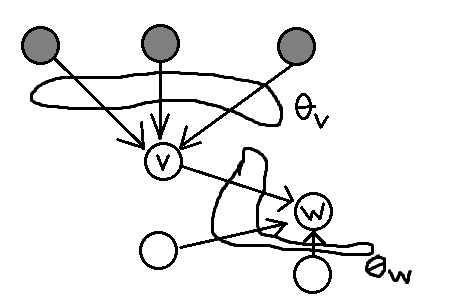
\includegraphics[width=\textwidth]{Figures/linearThreshold}
		\caption{Step 1 } 
		\label{fig:linearThresh}
	\end{subfigure}
	\begin{subfigure}{0.3\textwidth}
		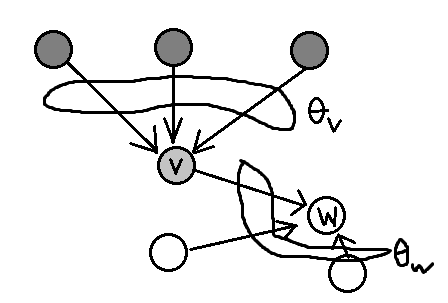
\includegraphics[width=\textwidth]{Figures/linearThreshold2}
		\caption{step 2 } 
		\label{fig:linearThresh2}
	\end{subfigure}
	\begin{subfigure}{0.3\textwidth}
		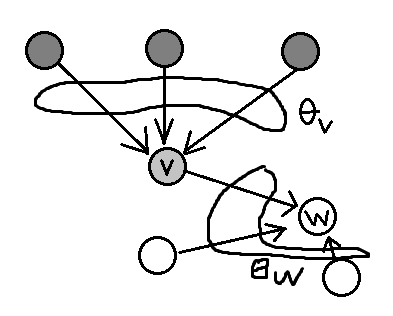
\includegraphics[width=\textwidth]{Figures/linearThreshold3}
		\caption{step 3} 
		\label{fig:linearThresh3}
	\end{subfigure}
	\caption{Linear Threshold mode}
\end{figure}

\subsection{Independent Cascade Model}
The independent cascade model (ICM) have a local or global probability for activation. In figure \ref{fig:ICM_step}, each node have their own local probability. In \ref{fig:ICM}, the node v is activated, during the next time-step, all of node vs neighbours use their internal probability to determine if they are activated or not. The result was three activation out of five. In the next time-step \ref{fig:ICM3} node w was able to activate the blue node. For a ICM with global probability, each node would then have the same probability to activate its neighbor. As we can see from Figure \ref{fig:ICM_step}, each neighbor to v is activated individually. As in \ref{fig:ICM2}, only three nodes were activated. In ICM, each node can only try to activate the neighbor once. In figure \ref{fig:ICM2}, the node that was not activated by v, got activated in \ref{fig:ICM3} by the node w.

%Fiks figur og tekst overfor.%
%Forlar hvordan ICM Funker%

\begin{figure}[!ht]
	\begin{subfigure}{0.3\textwidth}
		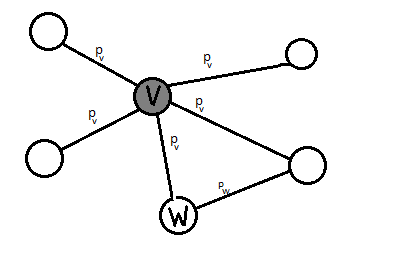
\includegraphics[width=\textwidth]{Figures/ICM}
		\caption{step 1 } 
		\label{fig:ICM}
	\end{subfigure}
	\begin{subfigure}{0.3\textwidth}
		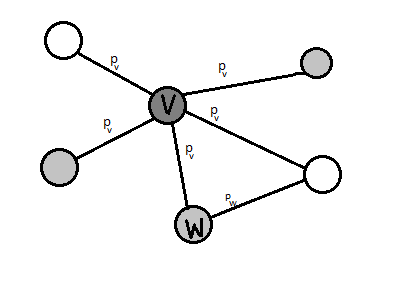
\includegraphics[width=\textwidth]{Figures/ICM2}
		\caption{step 2} 
		\label{fig:ICM2}
	\end{subfigure}
	\begin{subfigure}{0.3\textwidth}
		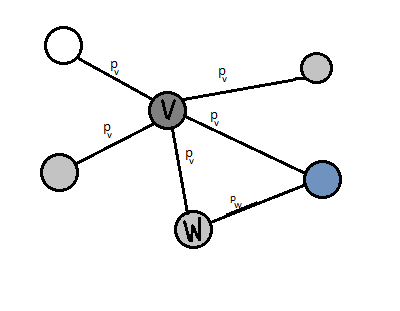
\includegraphics[width=\textwidth]{Figures/ICM3}
		\caption{step 3} 
		\label{fig:ICM3}
	\end{subfigure}
	\caption{Independent cascade model}
	\label{fig:ICM_step}
\end{figure}

We can compare the ICM with the same example we have been using, the cosmetic company promoting a product. Each new user have a chance(p$p_v$) to promote the product to a new user. The new user would then continue promoting the new product to his/hers friends. 

As mentioned earlier, the ICM is a special case of the breadth first search. If we set the transmisison probability to 1.0, meaning there are 100\% chance to activate the neighbores, the ICM is equal to BFS. BFS iterates through the graph by appending the child node not examined into the queue. Then examines a new node from the queue and repeating the process until all nodes have been examined. The main difference between the ICM and BFS, is that in ICM, there is a chance that the child node is not added into the queue. During each step, a random "coin toss" is tested to determent if the child node would be added into the queue. Other then that, both algorithms iterates through the network via edges.



 \section{Breadth First Search}
BFS is a tree traversal algorithm. BFS start at the root node \textit{$v_r$}. The algorithm then stores all $v_r$s children nodes in a \textit{queue}. The algorithm then takes the first node from the queue, \textit{$v_1$} and stores all the children nodes to \textit{$v_1$} in the back of the queue. This process continues until the queue is empty and all the nodes have been iterated over. 

BFS is a common graph iteration algorithm, but is often limited by the irregular memory access where the algorithm have to find the data stored in different spaces in memory.

%%forklar hva frontier er for noe
\begin{algorithm}
\caption{Breadth First Search}
\begin{algorithmic}[1]
\State{$dist[\forall \textit{v} \in V] = -1; currentQ, nextQ = \oldemptyset$}
\State $step = 0; dist[root] = step$
\State ENQUEUE(nextQ,root)
\While {$nextQ\neq \oldemptyset $}
\State $currentQ = newxtQ; nextQ = \oldemptyset$
\State $step = step+1$
\While {$currentQ \neq \oldemptyset$}
\State$ u$ = DEQUEUE(currentQ)
\For {$v \in Adj[u]$}
\If {$dist[v] == -1 $}
\State $dist[v] = step$
\State ENQUEUE(nextQ, v)
\EndIf
\EndFor
\EndWhile
\EndWhile
\Return dist
\end{algorithmic}
\end{algorithm}


 
\subsection{BFS to Data Diffusion}

The motivation for transforming breadth first search as matrix-vector multiplication is that displaying the graph algorithm as a matrix multiplication can display the data access pattern for the algorithm and can be readily optimized  \cite{AlgoToMath}.

As mentioned before, ICM is a special case of the breadth first search. By modifying the algorithm proposed earlier, we can in theory perform ICM with matrix-vector multiplication.  
\section{Matrix Notations}
Nodes and edges are not the only way to present a graph, graphs and networks can be represented as sparse adjacency matrices \cite{AlgoToMath}. We can see that such an idea have been proposed in earlier literature \cite{McAndrew1963}. By representing graphs as a sparse matrix, we can often discover different ways to optimize the algorithm, we can have a different structure to store data. The adjacency matrix in particular, is a interesting way to represent the graph. A graph $G =(V,E)$, G have N vertices and M edges, this correspond to a N$\times$N adjacency matrix called A. If A(i,j)=1, then there is an edge from $v_i$ to $v_j$. Otherwise its 0. In Figure:\ref{fig:AdjaToMatrix}, we can see how a undirected graph can be represented as an adjacency matrix. To generate a undirected graph as a adjacency matrix, the matrix must be mirrored diagonally, meaning if A(i,j)=1, then A(j,i)=1, if this is not true, then the matrix would be representing a directed graph.

\subsection{Sparse Matrix}
A sparse matrix is a matrix containing few nonzero. Social graph with few edges would often be represented as a sparse matrix. Since sparse matricies only have few non-zero elements, by storing only the non-zero elements, we can have savings in memory.

\begin{figure}
	\begin{subfigure}{0.5\textwidth}
	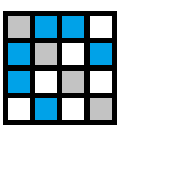
\includegraphics[width=\textwidth]{Figures/AdjacencyM}
	\caption{The adjacency matrix}
	\label{fig:AdjacencyM}
	\end{subfigure}
	\begin{subfigure}{0.5\textwidth}
	\includegraphics[width=\textwidth]{Figures/simpleGraph}
	\caption{The graph corresponding to the adjacency matrix}
	\label{fig:matrix}
	\end{subfigure}
 	\caption{Sparse matrix to graph}
 	\label{AdjaToMatrix}
\end{figure}

\subsection{Breadth First Search as Matrix Multiplication.} \label{BFS as Matrix}
From  \cite{AlgoToMath}, we can see that BFS can be recast as algebraic operations. BFS can be performed by applying matrix-vector multiplication over Boolean semirings \cite{HybridBFS2015}. The graph is represented as a adjacency matrix A, then for the root node, a vector x(root)=1 is multiplied with the matrix A. $A \times x_0 = y_0$. $y_0$ is the result after the first matrix-vector multiplication and in the next iteration, $x_1 = y_0$. We can see from the Figure\ref{fig:bfsMatrix}

\begin{figure}
	\includegraphics[width=\textwidth]{Figures/BFS_algo}
	\caption{BFS on Boolean semiring}
	\label{fig:bfsMatrix}
\end{figure}
\subsection{Semiring}
A $semiring$ is a set of elements with two binary operations. The two operations are often known as "addition"(+) and "multiplication"($\times$).  As we shown in previous section, the algorithm perform matrix multiplication uses the two operations, multiplications and addition. In  \cite{HybridBFS2015}, the AND and OR operator was chosen instead of the normal addition and multiplication. 

 
 
 \section{Seed Selection Algorithm}
The seed selection algorithm, is the algorithm used to select the initial $k$ seed nodes to be chosen at the start of the information diffusion. Each selected nodes is in the initial timestep activated. During each timestep, the seed nodes will propagate the activation along the network depend on what diffusion model is used. We can compare it to a new gadget or a cosmetic company trying to promote a new product. By selecting a few influential persons to give a free sample, the new trend would most likely  spread through $viral$ $marketing$ \cite{ViralMarketing}. The seed selection algorithm would be the algorithm to select the few influential individuals to receive this free sample. There are multiple different scheme to choose from, in this section, we will focus on four different algorithms, greedy algorithm, degree algorithm, random algorithm and the independent greedy algorithm.

\subsection{The Greedy Algorithm}
The greedy algorithm \cite{greedyInfluenc2005} proposed by Kempe et al, is known to be the best algorithm according to the result from  \cite{greedyInfluenc2005}. The greedy algotihm starts by itterate over the entire network and finds one node that have the largest coverage and stores that node in the set $A$. The algorithm then activates that node from A, and computes the coverage of each node in the network with the previous chosen node. After the algorithm finds the second node, that node is stored in A with the previous node and we have now chosen two seed node. The algorithm continues until we have choosen \textit{k} seed nodes, where each have been tested to have maximum coverage in relation with the previous chosen nodes. To compute the maximum coverage, the algorithm have to test every combination of nodes together, this results in heavy computation and the algorithm would therefore not scale well.

We can look at the greedy algorithm as a special case of BFS with a transistion probability. Each node in the network will be chosen as the seed node for the

 \begin{algorithm}
\caption{Greedy Algorithm}
\begin{algorithmic}[1]
\State Start with $A = \oldemptyset$
\While{$|A| \leq l$}
\State For each node $x$, use repeated sampling to approximate $\sigma(A \cup {x}) $ to within ($1 \pm \varepsilon$) with probability
$1 − \delta$
\State Add the node with largest estimate for $\sigma(A \cup {x})$ to A.
\EndWhile
\State Output the set $A$ of nodes.
\end{algorithmic}
\end{algorithm}

\subsection{The Degree Algorithm}
Another popular algorithm is the degree algorithm \cite{greedyInfluenc2005}. Unlike the greedy algorithm, does not compute the coverage of node, the algorithm picks the top \textit{k} nodes according to the degree distribution instead. The node chooses the top \textit{k} nodes with the highest degree and stores them as the seed nodes. This approach benefits over the greedy algorithm by not having as much computation time as the greedy algorithm since only one itteration is needed to compute the degree to node. The disadvantage is that this algorithm does not take the degree correlation into acount. As mentioned in section \ref{degreeCorr}, high degree nodes would often have common node as neighbor. This would result in multiple overlapping activated node choosen.

\begin{algorithm}
\caption{Degree Algorithm}
\begin{algorithmic}[1]
\State Start with $A = \oldemptyset$
\While{$|A| \leq l$}
\State For each node $x$, use repeated sampling to compute DegreeMax($x$).
\State Add the node with largest degree to A.
\EndWhile
\State Output the set $A$ of nodes.
\end{algorithmic}
\end{algorithm}

\subsection{Independent Algorithm}
Another algorithm is the independent greedy algorithm. The algorithm iterates through the network, computing the spread of each node. The algorithm then chooses the vertex with the largest coverage independent of the other previous chosen nodes. This algorithm is a special case of the greedy algorithm mentioned above.

\begin{algorithm}
\caption{Independent Algorithm}
\begin{algorithmic}[1]
\State Start with $A = \oldemptyset$
\While{$|A| \leq l$}
\State For each node $x$, use repeated sampling to approximate $\sigma(A \cup {x}) $ to within ($1 \pm \varepsilon$) with probability
$1 − \delta$
\State Add the node with largest estimate for $\sigma({x})$ to A.
\EndWhile
\State Output the set $A$ of nodes.
\end{algorithmic}
\end{algorithm}




\subsection{Random Algorithm}
The last one is the random algorithm. The random algorithm just picks a random seed node. This approach is the simplest to implement and easiest. The downside is that this is random and there are no strategic choosing of seed node. 

 
 
\section{High Level Synthesis}

High Level Synthesis converst algorithms implemented on higher level down to \textit{Register Transfer Level} (RTL)\cite{HLSTutorial}. RTL is models of digital circuits displaying flow of data between register, logical operations and such. It is commonly used to descripe low level digital systems. HLS is known to be able to reduce development effort and cost of creating specialized hardware compared to traditional hand-drawn RTL designs\cite{zhao2016improving}\cite{Zuo:2013:IHL:2435264.2435271}\cite{HLSTutorial}. By taking high level language such as C, C++ and SystemC implementations and generate the optimal architecture. HLS allows the user to generate custom \textit{Intellectual Property}(IP) core. An IP-core is a custom created data core that have an output and an input port.


\section{ZedBoard}
The Zedboard that we used for this project, is \textit{Xilinx Zynq-7000 All programmable System-on-chip(SoC)} Z-7020. Consist of a dual core \textit{ARM cortex-A9 MPCore} based processing system(PS) and an \textit{Artix-7 XC7Z020} FPGA. The FPGA is the \textit{programmable logic}(PL). The Zedboard have 512 MB DDR3 RAM, 256MB Quad-SPI Flash and 4GB SD card.\cite{FPGASoCManual}. The system offers the flexibility and scalability of an FPGA\citep{FPGAOVERVIEW}. 

THe FPGA use \textit{Advance eXtensible Interface}(AXI4)bus protocol. There are three types if AXI4 interfaces:
\begin{itemize}
\item \textbf{AXI4 Lite}- Simple, memory mapped communication. Useful for small single read.
\item \textbf{AXI4-Stream} - for continues streaming of data.
\item \textbf{AXI4} - For memory mapped applications.
\end{itemize} 

A component with PL implemented would be able to connect to the PS through a AXI4 bus port. The close coupling between t








\section{RMat} \label{rmat}
One problem during graph analyzation and calculation is finding suitable graphs to analyses. Generate graphs with desired properties is not easy to do. One solution proposed by Chakrabartiy et al is to use the "recursive matrix" or R-mat model. The R-mat model generates graph with only a few parameters, the generated graph will naturally have the small world properties and follows the laws of normal graphs, and have a quick generation speed \cite{Rmat2004}. The R-mat models goal is to generate graphs that matches the degree distribution, exhibits a " community " structure and have a small diameter and matches other criteria. \cite{Rmat2004}. The algorithm to generate such a recursive matrix is as follows: The idea is to partition the adjacency matrix into four equally sized part branded A,B,C,D, as shown in Figure\ref{fig:flipDiagonal}. The adjacency matrix starts by having all element set to 0. Each new edge is "dropped" onto the adjacency matrix. Which section the edge would be placed in, is chosen randomly. Each section have a probability of $\textit{a, b, c, d}$, and $a + b + c + d = 1$. After a section is chosen, the partition that was chosen is partitioned again. This continues until the chosen section is a 1x1 square and the edge is dropped there. From the algorithm, we can see that the R-mat generator are capable to generate graphs with total numbers of node $ \textit{V} = 2^x$. Since the algorithm partitioned the matrix into four part. This is approach would only generate a directed graph. To generate undirected graph, $b = c$ and the adjacency matrix must make a "copy flip" on the diagonal elements, like Figure \ref{fig:flipDiagonal}. 

\begin{figure}
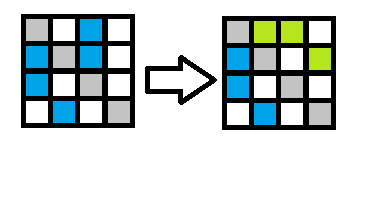
\includegraphics{Figures/flip_matrix}
\caption{How the adjacency matrix is flipped on the diagonal}
\label{fig:flipDiagonal}
\end{figure}